\chapter{Environment and Spacecraft Dynamics}

To test our hypothesis for the PARL+BC framework, we propose a constrained zero-sum game, initially based on linear-time-invariant 2nd-order HCW dynamics to model it like an interaction of two agents relative to a chief circular orbit in the Local-Vertical Local-Horizontal (LVLH) frame. We bound these agents into the boundary of an imaginary spherical in space arena centered at the chief of the orbit. In our initial setup, we have two agents and a static element in the environment:

\begin{enumerate}
\item \textbf{Asset/Object of Interest (OI):} A static object in the LVLH frame that is the "chief" of the orbit. 
\item \textbf{Player 1 (defender):} Defends an asset of interest by preventing player 2 from intercepting the asset of interest by capturing. If it intercepting player 2 or forces it out of the arena, it wins. 
\item \textbf{Player 2 (attacker):} Attacks the central chief asset of interest by preventing player 1's defense strategy. If it intercepts the asset of interest, forces the defender to crash into it, or forces the defender out of the arena, it wins.
\end{enumerate}

The result is an interesting variation of pursuit evasion scenario where the conditions above make it a zero sum, spatially constrained game that simplifies the learning for an online RL algorithm as is  PPO. Figure \ref{fig:3D_Rollout_Double} offers a visual depiction of the proposed game.

The states are the positions and velocities of each agent and the actions are continuous control inputs in 3D space, where we assume both spacecraft to be fully actuated in three translational degrees of freedom. For the sake of simplicity, we ignore the attitude evolution in this work, and we assume that the Player 1 and Player 2 are simply looking  at each other at all times.

The entire simulation environment was developed by the author of this thesis in Python, using full advantage of the PyTorch library to assist with the RL training. 

\begin{figure}[H]
    \centering
    \begin{minipage}{0.45\linewidth}
        \centering
        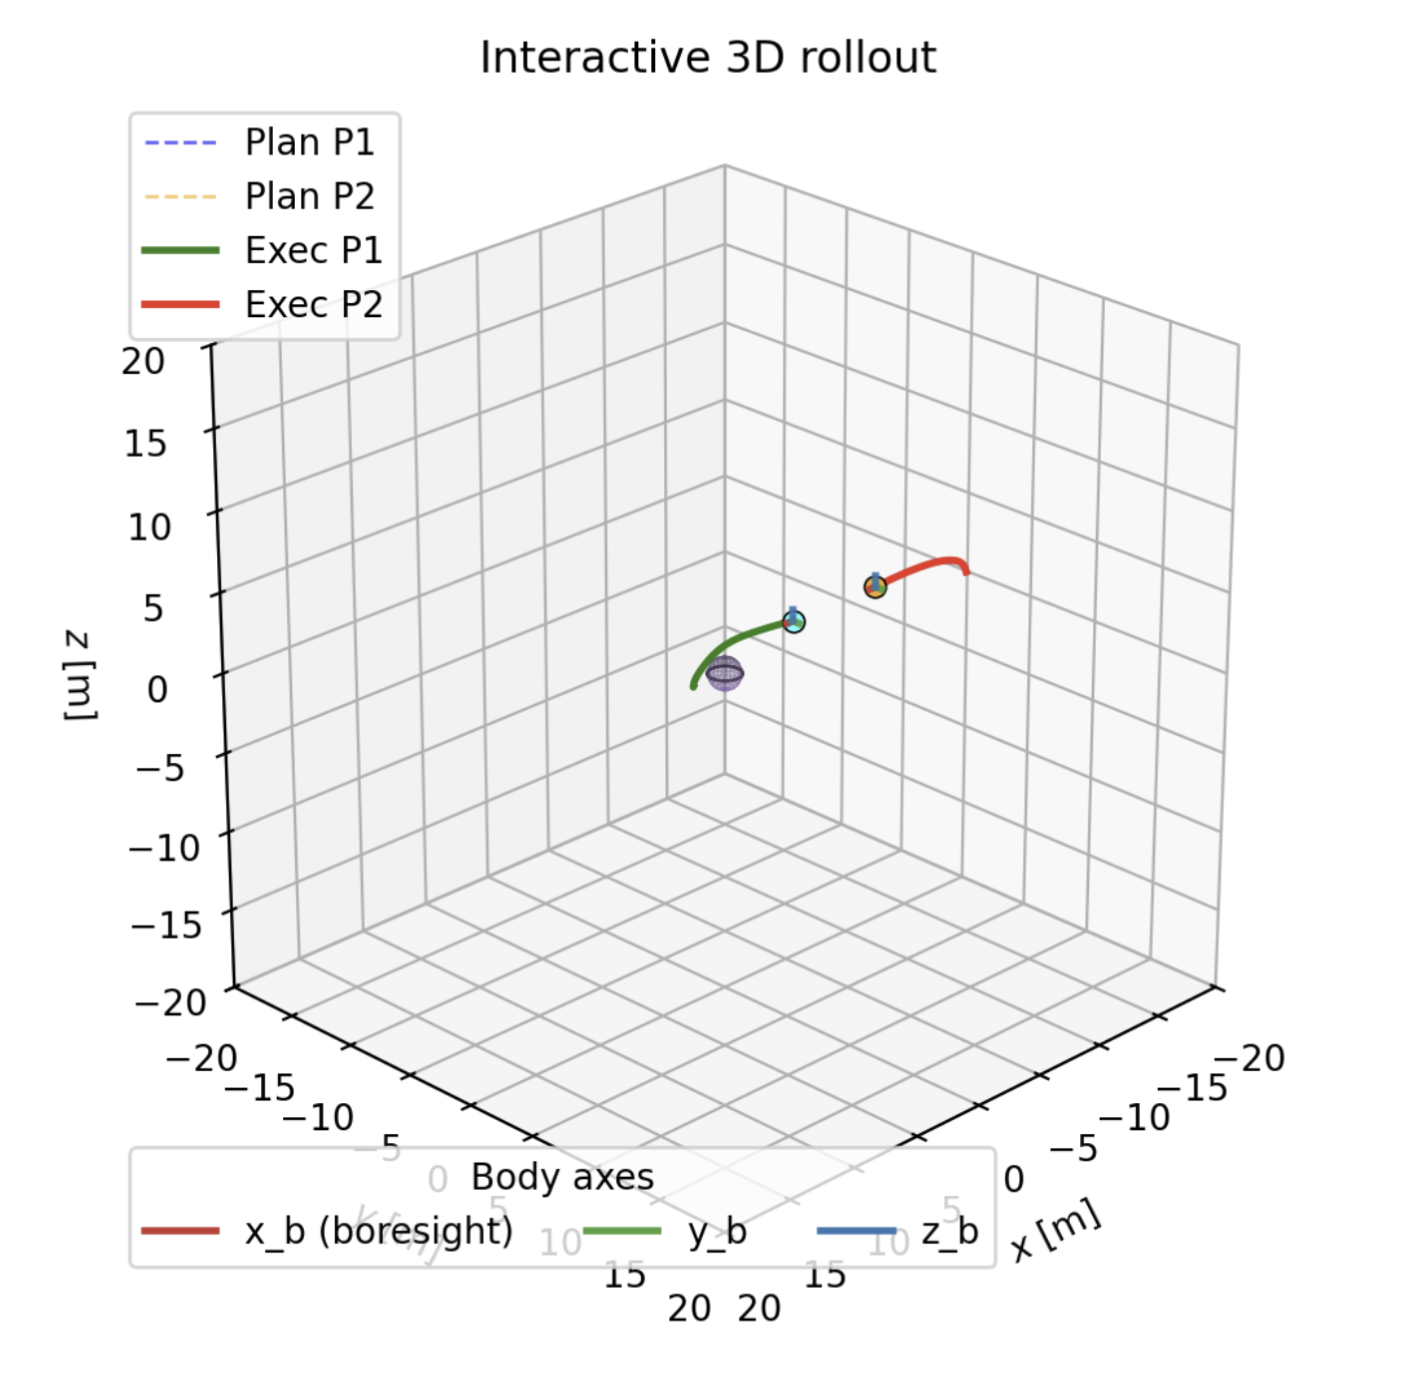
\includegraphics[width=\linewidth]{Figures/3D_Rollout.png}
    \end{minipage}
    % \hfill
    \begin{minipage}{0.45\linewidth}
        \centering
        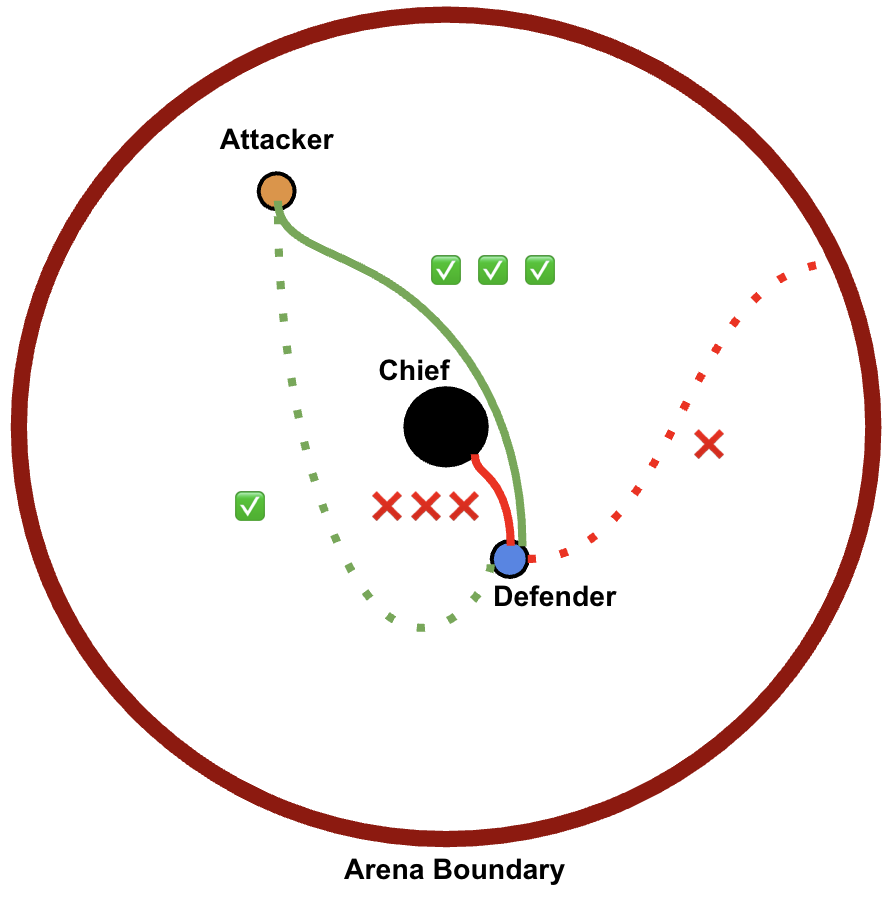
\includegraphics[width=\linewidth]{Figures/Training_Visulaization.png}
    \end{minipage}
    \caption{Sample of a policy rollout showing the agents carrying the proposed zero-sum game setup (left), as well as a simple graphic describing training scenarios for the defender (right).}
    \label{fig:3D_Rollout_Double}
\end{figure}



%===========
\newpage


\section{Dynamics models}

\subsection{HCW (Hill--Clohessy--Wiltshire) orbital relative dynamics - \cite{clohessy1960terminal} and \cite{hill1878researches}}

We model the follower in the chief agent's Local Vertical, Local Horizontal (LVLH) frame assuming a circular reference orbit of radius $r_0$ around a body with parameter $\mu$. The mean motion is defined as:
\[
n \;=\; \sqrt{\mu / r_0^3}
\]
Let $(x,y,z)$ be defined as the relative positions of the agents and let the control thrust acceleration of the agents be defined as:
$\vec{\mathbf{a}} = [a_x, a_y, a_z]^\top$.
For small separations between agents and assuming the chief follows a circular orbit, the linearized HCW equations are
\begin{align*}
\ddot{x} &= 2n \dot{y} + 3n^2 x  + a_x, \\
\ddot{y} &= - 2n \dot{x}            + a_y, \\
\ddot{z} &= - n^2 z                  + a_z
\end{align*}
Stacking the position and velocity elements into a single vector as 
$\vec{\mathbf{s}} := [x\ y\ z\ \dot{x}\ \dot{y}\ \dot{z}]^\top$
gives the linear time invariant (LTI) form:
\begin{gather*}
\dot{\vec{\mathbf{s}}} = F\vec{\mathbf{s}} + G\vec{\mathbf{a}},\\[4pt]
F =
\begin{bmatrix}
\mathbf{0}_{3\times3} & I_3\\[4pt]
\begin{array}{ccc}
3n^2 & 0   & 0\\
0    & 0   & 0\\
0    & 0   & -n^2
\end{array} &
\begin{array}{ccc}
0 & 2n & 0\\
-2n & 0 & 0\\
0 & 0 & 0
\end{array}
\end{bmatrix},
\quad
G =
\begin{bmatrix}
\mathbf{0}_{3\times3}\\[2pt]
I_3
\end{bmatrix}
\end{gather*}
With a sample time $\Delta t$, we do a zero order hold discretization as:
\begin{gather*}
A_d = e^{F\Delta t},\\[4pt]
B_d = \int_{0}^{\Delta t} e^{F\tau}\,G\,d\tau
\end{gather*}

From which we obtain our final dynamics evolution as:


\[
\vec{\mathbf{s}}_{k+1} = A_d\vec{\mathbf{s}}_k + B_d\vec{\mathbf{u}}_k,
\qquad
A_d \in \mathbb{R}^{6\times 6},
\quad
B_d \in \mathbb{R}^{6\times 3}
\]

Do note that HCW is globally Linear Time Invariant (LTI) here only under certain assumptions, which are sufficient given the scope of this research: that the chief agent is following a circular orbit, we're treating with small relative distances relative to the celestial object being orbited $\| (x,y,z)\| \ll r_0$, and that the control accelerations exerted by the agents are small relative to the central gravitational field.

\subsection{Elliptical LTV orbital relative dynamics - \cite{tschauner1965rendezvous}}

We have an elliptical dynamics model in order to study how our trained models behave under linear time variant dynamics. This means that instead of the A and B matrices remaining statics as they do with the HCW dynamics model, these A and B matrices change and evolve over time. Note that this model was used exclusively for Monte Carlo rollouts in this work, not for any of the trained policies.  

For this model, we again represent each agent in the chief's local frame. The main difference is that this time around we won't assume that the orbit is perfectly circular as we did in the HCW dynamics model. Instead, the chief follows an unperturbed Keplerian elliptical orbit with gravitational parameter $\mu$, semi-major axis $a$, eccentricity $e$, inclination $i$, right ascension of the ascending node $\Omega$, argument of periapsis $\omega$, and initial true anomaly $\nu_0$. 


The mean motion of the chief orbit is defined as:
\[
n \;=\; \sqrt{\mu/a^3}
\]
At a given time $t_k = k\Delta t$, the chief mean anomaly propagates as:
\[
M_k = M_0 + nt_k
\]
where $M_0$ is obtained from $\nu_0$. The eccentric anomaly $E_k$ is calculated from Kepler's equation:
\[
E_k - e\sin E_k = M_k
\]
and the corresponding true anomaly from the above is:
\[
\nu_k
=
2 \tan^{-1}
\left(
\frac{\sqrt{1+e}\sin(E_k/2)}
     {\sqrt{1-e}\cos(E_k/2)}
\right)
\]
The chief inertial position and velocity are then computed from its corresponding orbital elements. By defining:


\[
p = a(1-e^2),
\qquad
r_k = \frac{p}{1+e\cos\nu_k}
\]
the chief state then becomes:
\[
\vec{\mathbf{r}}_{c,p}
=
\begin{bmatrix}
r_k\cos\nu_k\\
r_k\sin\nu_k\\
0
\end{bmatrix},
\qquad
\vec{\mathbf{v}}_{c,p}
=
\sqrt{\frac{\mu}{p}}
\begin{bmatrix}
-\sin\nu_k\\
e+\cos\nu_k\\
0
\end{bmatrix}
\]
Then by using using the rotation matrix:
\[
Q = R_3(\Omega)R_1(i)R_3(\omega)
\]
we obtain the inertial chief state:
\[
\vec{\mathbf{r}}_{c,k} = Q\vec{\mathbf{r}}_{c,p}
\qquad
\vec{\mathbf{v}}_{c,k} = Q\vec{\mathbf{v}}_{c,p}
\]

At each time step, the chief's Radial--Transverse--Normal (RTN) frame is defined as:
\[
\hat{\vec{\mathbf{R}}}_k = \frac{r_{c,k}}{\|r_{c,k}\|},
\qquad
\hat{\vec{\mathbf{N}}}_k =
\frac{r_{c,k}\times v_{c,k}}
     {\|r_{c,k}\times v_{c,k}\|},
\qquad
\hat{\vec{\mathbf{T}}}_k = \hat{\vec{\mathbf{N}}}_k \times \hat{\vec{\mathbf{R}}}_k
\]

Here, we let the concatenated matrix:
\[
C_{RTN\to I,k}
=
\begin{bmatrix}
\hat{\vec{\mathbf{R}}}_k & \hat{\vec{\mathbf{T}}}_k & \hat{\vec{\mathbf{N}}}_k
\end{bmatrix}
\]

map RTN coordinates into inertial coordinates. The angular velocity of the RTN frame is then:
\[
\vec{\boldsymbol{\omega}}_k =
\begin{bmatrix}
0\\
0\\
\|\vec{\mathbf{r}}_{c,k}\times \vec{\mathbf{v}}_{c,k}\|/\|\vec{\mathbf{r}}_{c,k}\|^2
\end{bmatrix}
\]

Now, let the relative RTN position and velocity be
\[
\vec{\boldsymbol{\rho}} =
\begin{bmatrix}
\rho_R\\
\rho_T\\
\rho_N
\end{bmatrix},
\qquad
\dot{\vec{\boldsymbol{\rho}}} =
\begin{bmatrix}
\dot{\rho}_R\\
\dot{\rho}_T\\
\dot{\rho}_N
\end{bmatrix}
\]
and then define the stacked state of the agent as:

\[
\vec{\mathbf{s}} :=
\begin{bmatrix}
\rho_R &
\rho_T &
\rho_N &
\dot{\rho}_R &
\dot{\rho}_T &
\dot{\rho}_N
\end{bmatrix}^{\top}
\]

For a given control acceleration $
\vec{\mathbf{u}}_k = [u_R, u_T, u_N]^\top$ expressed in RTN coordinates, the inertial state of the deputy at any given time $t_k$ is:
\[
\vec{\mathbf{r}}_{d,k} = \vec{\mathbf{r}}_{c,k} + C_{RTN \to I,k}\vec{\boldsymbol{\rho}}_k
% r_{d,k}
% =
% r_{c,k}
% +
% C_{RTN\to I,k}\rho_k,
\]
\[
% v_{d,k}
% =
% v_{c,k}
% +
% C_{RTN\to I,k}
% \left(
% \dot{\rho}_k + \omega_k \times \rho_k
% \right)
\vec{\mathbf{v}}_{d,k} = \vec{\mathbf{v}}_{c,k} + C_{RTN \to I,k}(\dot{\vec{\boldsymbol{\rho}}}_k + \vec{\boldsymbol{\omega}}_k \times \vec{\boldsymbol{\rho}}_k)
\]
The deputy is then propagated over a single sample interval by using two-body inertial dynamics:
\[
\dot{\vec{\mathbf{r}}}_d = \vec{\mathbf{v}}_d,
\qquad
% -\mu\frac{r_d}{\|r_d\|^3}
% +
% C_{RTN\to I,k}u_k,
\dot{\vec{\mathbf{v}}}_d = -\mu \frac{\vec{\mathbf{r}}_d}{ \|\vec{\mathbf{r}}_d\|^3} + C_{RTN \to I,k}\vec{\mathbf{u}}_k,
\]
where the control acceleration held constant over the interval on a zero-order hold.

Following the propagation to $t_{k+1}$, the inertial deputy state is then transformed back into the new chief's RTN frame:
\[
\vec{\boldsymbol{\rho}}_{k+1}
=
C_{I\to RTN,k+1}
\left(
\vec{\boldsymbol{r}}_{d,k+1}-\vec{\boldsymbol{r}}_{c,k+1}
\right),
\]
\[
\dot{\vec{\boldsymbol{\rho}}}_{k+1}
% \dot{\rho}_{k+1}
=
C_{I\to RTN,k+1}
\left(
\vec{\boldsymbol{v}}_{d,k+1}-\vec{\boldsymbol{v}}_{c,k+1}
\right)
-
\vec{\boldsymbol{\omega}}_{k+1}\times \vec{\boldsymbol{\rho}}_{k+1}.
\]
This transformation defines a nonlinear discrete-time map:
\[
% s_{k+1} = f_k(s_k,u_k)
\vec{\mathbf{s}}_{k+1} = f_k(\vec{\mathbf{s}}_k, \vec{\mathbf{u}}_k)
\]


For the rollout model of the policies into this elliptical model, we use a linear time-varying approximation of this map about the chief trajectory. In other words, an approximation about zero relative state and zero control:
\[
\vec{\mathbf{s}}_k = \vec{\mathbf{0}},
\qquad
\vec{\mathbf{u}}_k = \vec{\mathbf{0}}
\]
The discrete LTV matrices are then computed on each step as:
\[
A_k
=
\left.
\frac{\partial f_k}{\partial s}
\right|_{s=0,u=0},
\qquad
B_k
=
\left.
\frac{\partial f_k}{\partial u}
\right|_{s=0,u=0}.
\]
In this implementation, these Jacobians are obtained by using centered finite differences in the form:
\[
A_k[:,j]
\approx
\frac{
f_k(\epsilon e_j,0) - f_k(-\epsilon e_j,0)
}{2\epsilon},
\qquad
j=1,\ldots,6,
\]
\[
B_k[:,j]
\approx
\frac{
f_k(0,\epsilon e_j) - f_k(0,-\epsilon e_j)
}{2\epsilon},
\qquad
j=1,\ldots,3.
\]
And finally, the rollout dynamics are therefore:
\[
\vec{\mathbf{s}}_{k+1} = A_k\vec{\mathbf{s}}_k + B_k\vec{\mathbf{u}}_k,
\qquad
A_k \in \mathbb{R}^{6\times 6},
\quad
B_k \in \mathbb{R}^{6\times 3}.
\]

which define the time evolution of the state in the same way we did with HCW, but using our new elliptical dynamics model.

Unlike HCW dynamics, however, the model is clearly not globally Linear Time Invariant (LTI) since the chief's orbital radius, true anomaly, and RTN frame angular rate vary along the elliptical orbit. This approximation is valid for small relative separation relative to the chief's orbital radius, control accelerations that are smaller relative to the central gravitational field, and assuming that the Keplerian chief trajectory remains unperturbed.

\subsection{Orbits used in this work}

Throughout this thesis, whenever we refer to HCW and Elliptical LTV dynamcis we refer to just one chief orbit per dynamics model to exemplify each case within the context of the work. The commanded motion each agent undergoes then occurs relative to this chief orbit. The parameters of each of these orbits are:

\begin{table}[H]
\centering
\caption{Chief orbit parameters used for the HCW and elliptic LTV dynamics.}
\label{tab:chief-orbit-parameters}
\begin{tabular}{lcc}
\toprule
\textbf{Parameter} & \textbf{HCW circular orbit} & \textbf{Elliptic LTV orbit} \\
\midrule
Use case & Training and evaluation & Evaluation only \\
Radius / semi-major axis & $r_0 = 6771~\mathrm{km}$ & $a = 7646~\mathrm{km}$ \\
Eccentricity & $e = 0$ & $e = 0.0948$ \\
Perigee altitude & $400~\mathrm{km}$ & $550~\mathrm{km}$ \\
Apogee altitude & $400~\mathrm{km}$ & $2000~\mathrm{km}$ \\
Orbital period & $92.41~\mathrm{min}$ & $110.89~\mathrm{min}$ \\
\bottomrule
\end{tabular}
\end{table}

And the following is a visualization for these:

\begin{figure}[H]
    \centering
    
\includegraphics[width=0.9\linewidth]{Figures/Merged_Thesis/chief_orbit_hcw_vs_elliptic_ltv.png}
    \caption{Chief orbit geometry used for the HCW and elliptic LTV dynamics, showing the circular training/evaluation orbit and the elliptic evaluation-only orbit.}
    \label{fig:Orbits_Visualization}
\end{figure}




\section{Estimation model - Bearing-Only Extended Kalman Filter (EKF)}

An bearings-only EKF model, based on the work in \cite{aidala1979kalman} which is based on the foundational piece by \cite{kalman1960new}, was picked for our state estimation architecture. This bearings-only EKF basically takes azimuth-elevation measurements (essentially acting as a basic optical navigation suite). Ergo, the measurement model is non-linear, even if the dynamics model may be linearized as is the case with HCW. Algorithm \ref{alg:kf-methodology} describes the step of the KF measurement and update process:




% Drop-in snippet for papers using \usepackage{algorithm} and \usepackage{algpseudocode}
\begin{algorithm}[H]
\caption{Agent-Centric Bearing-Only Kalman Filter Update}
\label{alg:kf-methodology}
\begin{algorithmic}[1]
\State \textbf{Given:} HCW dynamics $(A,B)$, step size $\Delta t$, measurement period $m$, process noise $Q$, measurement noise $R$
\State \textbf{Initialize the agent beliefs:}
\State \hspace{1em} Initialize defender belief over attacker $(\hat{\vec{\mathbf{x}}}^{D \to A}_0 ,P^{D\to A}_0)$ and attacker belief over defender $(\hat{\vec{\mathbf{x}}}^{A \to D}_0P^{A\to D}_0)$
\State \textbf{Define the measurement model:}
\State \hspace{1em} For observer $i$ and target $j$, let:
\[
% d_t^{i\to j}=p_t^j-p_t^i
\vec{\mathbf{d}}^{i \to j}_t = \vec{\mathbf{p}}^j_t - \vec{\mathbf{p}}^i_t ,\quad
\vec{\mathbf{b}}^{i \to j}_t = \frac{R^i_{wb}\vec{\mathbf{d}}^{i \to j}_t}{\|\vec{\mathbf{d}}^{i \to j}_t\|^2},\quad
h(\vec{\mathbf{p}}_t^i, R_{wb}^i, \vec{\mathbf{p}}_t^j)=
\begin{bmatrix}
\mathrm{atan2}(b_{y,t}^{i\to j},\,b_{x,t}^{i\to j})\\[2pt]
\mathrm{atan2}\!\big(b_{z,t}^{i\to j},\,\sqrt{(b_{x,t}^{i\to j})^2+(b_{y,t}^{i\to j})^2}\big)
\end{bmatrix}
\]
\For{$t=1,\dots,T$}
  \State \textbf{Propagate the true defender and attacker states:}
  \State \hspace{1em} Apply controls $\vec{\mathbf{u}}^D_t,\vec{\mathbf{u}}^A_t$
  \For{each observer-target pair $(i,j)\in\{(D,A),(A,D)\}$}
    \State \textbf{Select the filter control input:}
    \State \hspace{1em} $\tilde{\vec{\mathbf{u}}}^j_t\leftarrow \texttt{action\_access}$
    \State \textbf{Predict the belief mean and covariance:}

 \State \hspace{1em} $\hat{\vec{\mathbf{x}}}_{t|t-1}^{i\to j}\leftarrow A\hat{\vec{\mathbf{x}}}_{t-1|t-1}^{i\to j}+B\tilde{\vec{\mathbf{u}}}_t^j;\qquad
P_{t|t-1}^{i\to j}\leftarrow A P_{t-1|t-1}^{i\to j} A^\top + Q + B\Sigma_u B^\top$
    \If{$t \bmod m = 0$}
      \State \textbf{Form the noisy bearing measurement:}
      \State \hspace{1em} $\vec{\mathbf{z}}^{i \to j}_t\leftarrow h(\vec{\mathbf{p}}_t^i, R_{wb}^i, \vec{\mathbf{p}}_t^j)=+\nu_t$, $\nu_t\sim\mathcal{N}(0,R)$
      \State \textbf{Apply the EKF correction:}
      \State \hspace{1em} Linearize $h$, compute innovation $\vec{\mathbf{y}}^{i \to j}_t = \vec{\mathbf{z}}^{i \to j}_t - \hat{\vec{\mathbf{z}}}^{i \to j}_{t|t-1}$, update  belief
      \State \textbf{Log the innovation and covariance diagnostics:}
      \State \hspace{1em} Log $\|\vec{\mathbf{y}}_t^{i\to j}\|_2^2$ and $\mathrm{tr}(P^{i\to j}_{t,\mathrm{pos}})$
    \EndIf
    \If{belief diverges or leaves the allowed radius bound}
      \State \textbf{Repair the divergent belief:}
      \State \hspace{1em} Clip/reset belief and restore covariance to $P_0$
    \EndIf
  \EndFor
  \State \textbf{Build the agent observations from truth and belief:}
  \State \hspace{1em} Use true self-state and estimated opponent state
  \State \textbf{Compute reward and termination from the true physical state:}
  \State \hspace{1em} Evaluate reward and terminal conditions from the true propagated state
\EndFor
\State \textbf{Return the final beliefs and belief-space observations:}
\State \hspace{1em} $(\hat{\vec{\mathbf{x}}}^{D\to A}_{T|T},P^{D\to A}_{T|T})$, $(\hat{\vec{\mathbf{x}}}^{A\to D}_{T|T},P^{A\to D}_{T|T})$, and resulting belief-space agent observations
\end{algorithmic}
\end{algorithm}


Note that the EKF needs the opponent's action $\tilde{u}_t^j$ during training and rollout. If this is set to none, the state measurement quality degrades significantly, and early testing of action-less KF policies showed that it produced completely incoherent policies in partial observability. Therefore, one of the big assumptions we make in this research is that, any agent has somehow measured their adversaries action using some other means, recovering the noiseless ground state with no noise or the ground state within a Gaussian noise profile.

While an Unscented Kalman Filter (UKF)  would be more friendly to further sensor fusion within the proposed architecture, an EKF was picked given that early testing of our estimation-in-the-loop training signaled to extremely long training times (on the order of days of training time per phase) with a UKF in the loop, likely due to the high compute utilization of the unscented transform. Furthermore, EKFs are more common seen in real-life aerospace estimation architectures.


\section{Controller model - CBF-QP velocity saturation controller}

One of the later additions to this research was the implementation of a CBF-QP controller (\cite{ames2017control}) to saturate the velocities of the agents during training and rollout.

There's a couple reasons behind this addition. First of all, we discovered during earlier development of this research that, without the velocity saturation limit, the agents would become greedy and myopic with the access they had to their own control output commands. The result of this was that the agents, especially the defender, would pick up a lot of speed by using most of the control limit and then struggle to steer and control themselves during training and rollout. 

Therefore, we decided to implement velocity saturation for both agents into our system, both during training and evaluation. For practical purposes, this velocity saturation can be justified as a safety barrier, one that bounds the velocities of the agents to avoid unsafe speeds at which they could collide and cause significant damage to each other, which is not the intent of the proposed game.

One route we considered to implement this was to include a velocity/control saturating element in the reward function described in section \ref{sec:Rewards/Termination}, which would have been possible but we would have lost interpretability of the reward function and the mean reward return during training by combining various elements with different units into one monolithic reward function. Generally speaking, as we mention throughout that section, we found our RL trainings to behave best the simpler and cleaner our reward shaping was.

Therefore, to fill in this gap, we saw this as a great opportunity to show how a classical controller could fill in this gap and do this velocity saturation relative to a predefined max velocity $v_{max}$. We opted to use a CBF-QP, which filters the commanded action relative to whether it's considered feasible within the set defined by the velocity constraint. If the state is safe and the QP is feasible, then the system keeps the overall spacecraft dynamics within that set. If it is unfeasible, however, the filter will only return the least-violating admissible action. This would correspond to situations where the commanded correction to remain within the bounds of $v_{max}$ is incompatible with the available control authority.

The RL-trained policies are directly affected and have to adapt to this new filter as it becomes a part of the environment the Markov chain needs to adjust to. In other words, the policy has to learn from a pre-filtered environment where $u_{nom}$ is not really the applied action. Rather, the safety layer of the CBF-QP changes the overall transition map used throughout the learning. This, in turn, keeps the learning setup Markov, at least on the full-state case, as it keeps the applied control as a deterministic function of the current state and its commanded action. 

The massive benefit of this is that the CBF-QP safety filter does not introduce any hidden dynamics into the controls system or the training logic. Rather, it modifies the environment learning transition map from one that would learn under raw policy commands without it to one that learns under the CBF-QP-filtered commands. This, in turn, ends up providing a computationally efficient constraint on the agents' velocities while allowing the training logic to remain as simple as possible by not having to focus on anything other than the relative distances between the agents and the asset exclusively.

 Overall, the CBF-QP was highly performing during training and rollout right from its implementation, successfully constraining the net agent speed while not noticeably interfering on the agent's learning or compute speeds during training or evaluation. The process is described in detail in algorithm \ref{alg:velocity-cbf-qp}.

% Drop-in snippet for papers using \usepackage{algorithm} and \usepackage{algpseudocode}


\begin{algorithm}[H]
\caption{Velocity CBF-QP Saturation Filter}
\label{alg:velocity-cbf-qp}
\begin{algorithmic}[1]
\State \textbf{Given:} nominal action $\vec{\mathbf{u}}_t^{\mathrm{nom}}$, agent state $(\vec{\mathbf{p}}_t,\vec{\mathbf{v}}_t)$, box bounds $-u_{\max}\le \vec{\mathbf{u}}\le u_{\max}$, speed limit $v_{\max}$, CBF gain $\alpha$, HCW mean motion $n$
\State \textbf{Compute the barrier value:}
\State \hspace{1em} $h_t \leftarrow v_{\max}^2-\|\vec{\mathbf{v}}_t\|_2^2$
\State \textbf{Compute the HCW drift in the velocity channel:}
\State \hspace{1em}
\[
\vec{\mathbf{f}}_v(\vec{\mathbf{p}}_t,\vec{\mathbf{v}}_t)\leftarrow
\begin{bmatrix}
3n^2 p_{x,t}+2n v_{y,t}\\
-2n v_{x,t}\\
-n^2 p_{z,t}
\end{bmatrix}
\]
\State \textbf{Form the CBF half-space from $\dot h_t+\alpha h_t\ge 0$:}
\State \hspace{1em}
\[
\vec{\mathbf{a}}_t \leftarrow 2\vec{\mathbf{v}}_t,\qquad
b_t \leftarrow \alpha h_t - 2 \vec{\mathbf{v}}_t^\top \vec{\mathbf{f}}_v(\vec{\mathbf{p}}_t,\vec{\mathbf{v}}_t)
\]
\State \textbf{Pose the box-constrained projection:}
\State \hspace{1em}
\[
\vec{\mathbf{u}}_t^\star \leftarrow
\arg\min_{\vec{\mathbf{u}}}\ \tfrac12\|\vec{\mathbf{u}}-\vec{\mathbf{u}}_t^{\mathrm{nom}}\|_2^2
\quad\text{s.t.}\quad
\vec{\mathbf{a}}_t^\top \vec{\mathbf{u}} \le b_t,\ \ -u_{\max}\le \vec{\mathbf{u}}\le u_{\max}
\]
\State \textbf{Check whether the clipped nominal action is already feasible:}
\State \hspace{1em} Clip $\vec{\mathbf{u}}_t^{\mathrm{nom}}$ to the box bounds; if the clipped action already satisfies $\vec{\mathbf{a}}_t^\top \vec{\mathbf{u}} \le b_t$, return it
\State \textbf{Construct the box corner that minimizes the half-space left-hand side:}
\State \hspace{1em} Let $\vec{\mathbf{u}}_{\min}$ have components $(u_{\min})_k=-u_{\max}$ if $(a_t)_k\ge 0$ and $(u_{\min})_k=+u_{\max}$ otherwise
\State \textbf{Handle the infeasible case:}
\State \hspace{1em} If $\vec{\mathbf{a}}_t^\top \vec{\mathbf{u}}_{\min}>b_t$, return the least-violating box action $\vec{\mathbf{u}}_t^\star\leftarrow \vec{\mathbf{u}}_{\min}$
\State \textbf{Otherwise search the KKT multiplier:}
\State \hspace{1em}
\[
\vec{\mathbf{u}}(\lambda)\leftarrow \mathrm{clip}\!\big(\vec{\mathbf{u}}_t^{\mathrm{nom}}-\lambda \vec{\mathbf{a}}_t,\ -u_{\max},\ u_{\max}\big)
\]
\State \textbf{Bracket and bisect $\lambda$:}
\State \hspace{1em} Increase $\lambda$ until $\vec{\mathbf{a}}_t^\top \vec{\mathbf{u}}(\lambda)\le b_t$, then bisect on $\lambda$ to the desired tolerance
\State \textbf{Return the projected feasible action:}
\State \hspace{1em} $\vec{\mathbf{u}}_t^\star \leftarrow \vec{\mathbf{u}}(\lambda)$
\end{algorithmic}
\end{algorithm}


\section{State, action, and observation.}


Consider two agents described at the beginning of this chapter, a defender which we refer to as player/agent \#1 and an attacker which we refer to as player/agent \#2. These agents evolve under discretized dynamics (e.g: HCW), relative to a chief orbit, with a discrete time sampling \(\Delta t\).
For each agent \(i\in\{1,2\}\), their state is defined as:


\[
\vec{\mathbf{x}}_i =
\begin{bmatrix}
\vec{\mathbf{p}}_i\\
\vec{\mathbf{v}}_i
\end{bmatrix}\in\mathbb{R}^{2D},\quad
\vec{\mathbf{x}}_i^+ = A_d\vec{\mathbf{x}}_i + B_d\vec{\mathbf{u}}_i,\quad\vec{\mathbf{u}}_i\in\mathbb{R}^{D}
\]

where \(p_i,v_i\in\mathbb{R}^{D}\) are the agents position and velocity in the relative frame and \(u_i\) is a commanded acceleration clipped to a system actuation bound \(\|u_i\|_\infty\le u_{\max}\).
With this in mind, the concatenated state for the environment is defined as \(s=\big[x_1^\top,\,x_2^\top\big]^\top\in\mathbb{R}^{4D}\).

Each policy observes a fixed, task-shaped observation vector defined as:
\begin{equation}
\label{eq:Full_Obs_Both_Agents}
\boxed{
\vec{\mathbf{o}} = [(\vec{\mathbf{p}}_1-\vec{\mathbf{c}}),(\vec{\mathbf{p}}_2-\vec{\mathbf{c}}), (\vec{\mathbf{p}}_2-\vec{\mathbf{p}}_1), \vec{\mathbf{v}}_1, \vec{\mathbf{v}}_2]
}
\end{equation}


Which for the partially observable settings become the following for the attacker:

\begin{equation}
\label{eq:EKF_Obs_Agent_1}
\boxed{
\vec{\mathbf{o}}_{1,EKF} = [(\vec{\mathbf{p}}_1-\vec{\mathbf{c}}), (\tilde{\vec{\mathbf{p}}}_{2,1}-\vec{\mathbf{c}}), (\tilde{\vec{\mathbf{p}}}_{2,1}-\vec{\mathbf{p}}_1), \vec{\mathbf{v}}_1, \tilde{\vec{\mathbf{v}}}_{2,1}]
} 
\end{equation}


And the following for the defender:

\begin{equation}
\label{eq:EKF_Obs_Agent_2}
\boxed{
\vec{\mathbf{o}}_{2,EKF} = [(\tilde{\vec{\mathbf{p}}}_{1,2}-\vec{\mathbf{c}}), (\vec{\mathbf{p}}_2-\vec{\mathbf{c}}), (\vec{\mathbf{p}}_2-\tilde{\vec{\mathbf{p}}}_{1,2}), \tilde{\vec{\mathbf{v}}}_{1,2}, \vec{\mathbf{v}}_2]
}
\end{equation}

Where the quantities with tilde are those measured  via the bearings-only EKF described in algorithm \ref{alg:kf-methodology}. 

For the fully observable setting, we model the proposed zero-sum game as a discrete-time Markov Decision Process (MDP, for short). Here, the state consists of the previously laid out spacecraft states, the action is the agents' commanded control in 3D, and the transition map is provided and filtered by the spacecraft dynamics and the CBF-QP controller logic. The reward function and termination conditions are defined by the game's objectives as described in section \ref{}. For the partially obsevable setting via behavior cloning, the full-state MDP is replaced by the bearings only EKF measurement-based approximation, where the agents act based on the measurements they can get of their opponent instead of having access to its full state.


One future area for development on the partial observability setting would be the implementation of a self-estimation model from which each agent also has to estimate their own position in space (e.g: essentially using an IMU model), which would add another layer of realism to the research presented in this work. Given the already high degree of complexity of the current research, we decided to not pursue that direction in this work.



\section{Reward shaping and termination conditions}
\label{sec:Rewards/Termination}

We then gather the distances of each agent to the center and their relative distance and normalize relative to the radius of the arena \(R\) and a constant colission radius $r_{\text{collision}}$. We use these to define define the unitless attacker-to-center $d_1$, defender-to-center $d_2$, and docking distance $d_{\text{dock}}$. Note that these normalizations are absolutely necessary, as they provide stability during training. Upon normalizing, these quantities become:
\[
d_1 = \frac{\|\vec{\mathbf{p}}_1-\vec{\mathbf{c}}\|^2}{R^2},\qquad
d_2 = \frac{\|\vec{\mathbf{p}}_2-\vec{\mathbf{c}}\|^2}{R^2},\qquad
d_{dock} = \frac{\max(0, \|\vec{\mathbf{p}}_2-\vec{\mathbf{p}}_1\| - r_{collision})}{R}
\]



Note that unitless quantity $d_{\text{dock}}$ is not squared unlike unitless quantities $d_1$ and $d_2$ on purpose, as during our game it is meant to be a correcting factor, and $d_1$ and $d_2$ are supposed to be the dominating terms. 

Using these, we finally define our reward function for each time step, which for the defender is simply defined as:

% \[
% \boxed{
% \begin{aligned}
% r_1
% = {}&
% \underbrace{k_{\text{pos}}\, d_2}_{\substack{\text{encourage}\\\text{attacker}\\\text{away from}\\\text{asset}}}
% -
% \underbrace{k_{\text{dock}}\, d_{\text{dock}}}_{\substack{\text{penalize}\\\text{large}\\\text{defender--attacker}\\\text{separation}}}
% \end{aligned}
% }
% \]

\begin{equation}
\label{eq:attacker_step_reward}
\boxed{
\begin{aligned}
r_1
= {}&
\underbrace{k_{\text{pos}}\, d_2}_{\substack{\text{encourage attacker}\\\text{away from}\\\text{asset}}}
-
\underbrace{k_{\text{dock}}\, d_{\text{dock}}}_{\substack{\text{penalize large}\\\text{defender--attacker}\\\text{separation}}}
\end{aligned}
}
\end{equation}


% \[
% \boxed{
% \begin{aligned}
% r_1
% = {}&
% \underbrace{k_{\text{pos}}\, d_2}_{\text{encourage attacker away from asset}}
% \end{aligned}
% }
% \]

And with episodic terminal rewards defined as:

\begin{itemize}
    \item $r_1$ += $\beta_{intercept}$ for intercepting/docking to the attacker.
    \item $r_1$ += $\beta_{wall}$ for forcing the attacker out of the arena.
    \item $r_1$ -= $\beta_{intercept}$ for defender crashing onto the asset of interest.
    \item $r_1$ -= $\beta_{wall}$ for defender leaving the arena.
    
\end{itemize}

And in order to keep the game as a min-max zero sum, the attacker reward is simply: 

\[
\boxed{
\begin{aligned}
r_2
= {}&
\underbrace{-r_1}_{\text{attacker reward function}}
\end{aligned}
}
\]

So laid out this turns out to be a reward function in the form:

\begin{equation}
\label{eq:defender_step_reward}
\boxed{
\begin{aligned}
r_2
= {}&
\underbrace{-k_{\text{pos}}\, d_2}_{\substack{\text{encourage attacker}\\\text{towards}\\\text{asset}}}
+
\underbrace{k_{\text{dock}}\, d_{\text{dock}}}_{\substack{\text{reward large}\\\text{defender--attacker}\\\text{separation}}}
\end{aligned}
}
\end{equation}

And with episodic terminal rewards defined as:

\begin{itemize}
    \item $r_1$ -= $\beta_{intercept}$ for intercepting/docking to the attacker.
    \item $r_1$ -= $\beta_{wall}$ for forcing the attacker out of the arena.
    \item $r_1$ += $\beta_{intercept}$ for defender crashing onto the asset of interest.
    \item $r_1$ += $\beta_{wall}$ for defender leaving the arena.
    
\end{itemize}

\subsection{Partial observability via behavior cloning}

One must note that the partially observable policies corresponding to observations \ref{eq:EKF_Obs_Agent_1} and \ref{eq:EKF_Obs_Agent_2} also have access this form of a full state reward during training. This is because on the partially observable policies we want to purposefully match the measured observations to the full state reward, a process called behavior cloning, based on the work by \cite{ross2011reduction}.

In this process, we essentially create a measurement-based "student" that must learn from these fully observable rewards, with the intent of matching the behavior of the full state rewards as best as possible despite the sensor noise.

This process proves to be perhaps the simplest way to match sensor measurements to RL rewards, which is why it was chosen. There's other potential methods for training partially observable policies, such as distillation-based methods (e.g: \cite{bajcsy2024learning}). We looked into implementing these methods earlier on, but found them to be too computationally expensive, so we proceeded regular behavior cloning in this form. 
